%	!Mode::"UTF-8"
%	本模板设置改自北京大学交叉学院 王宇哲学长和北京大学化学与分子工程学院 王应泽同学的分享,特此感谢!
%	模板制作:北京大学化学与分子工程学院 王梓涵
%	Email:2100011837@stu.pku.edu.cn
%	本模板仅适用于北京大学物理化学实验报告,其他学校请自行修改
%	吐槽:Latex用于写物化实验报告还是过于繁琐了,不过还是比Word好用多了(๑•̀ㅂ•́)و✧ (此吐槽由copilot自动生成,模板作者认为word更好用)
%	本模板仅供交流学习使用,不可用作商业用途。

\documentclass[12pt]{article}

%	页面设置
\usepackage{geometry}
\geometry{left=2.5cm, right=2.5cm, top=2.5cm, bottom=2.5cm}
\usepackage{graphicx}
\usepackage{ctex}
\usepackage{fontspec}
\usepackage{setspace}
\usepackage[usenames,dvipsnames]{xcolor}
\usepackage{titlesec}

%	字体设置
\setmainfont{Times New Roman}
\setCJKmainfont{SimSun}
\setCJKsansfont{SimHei}

%	表格设置\
\usepackage{array,colortbl}
\usepackage{makecell}
\newcommand{\addcell}[2][4]{\makecell{\zihao{#1}\textsf{#2}}}
\usepackage{titlesec}
\usepackage{booktabs}
\usepackage{ragged2e} 
\usepackage{multirow}
\usepackage{tabularx}

%	设置图注、表注
\usepackage{caption}
\usepackage{bicaption}
\captionsetup{labelsep=quad, font={small, bf}, skip=2pt}
\DeclareCaptionOption{english}[]{
    \renewcommand\figurename{Fig.}
    \renewcommand\tablename{Table}
}
\captionsetup[bi-second]{english}

%	设置页眉
\usepackage{fancyhdr}
\usepackage{xpatch}
\pagestyle{fancy}
\fancypagestyle{preContent}{
    	\fancyhead[L]{\zihao{-5} 物理化学实验}
    	\fancyhead[C]{\zihao{-5} 实验十\ \ 磁化率的测定}
    	\fancyhead[R]{\zihao{-5} 2100011837\ 王梓涵}
		\renewcommand{\headrulewidth}{2pt}
		\renewcommand{\footrulewidth}{1pt}
		\xpretocmd\headrule{\color{BrickRed}}{}{\PatchFailed} % 设置页眉分割线颜色
		\xpretocmd\footrule{\color{BrickRed}}{}{\PatchFailed} % 设置页脚分割线颜色
}
\pagestyle{preContent}



%	设置首页页眉及取消首页页脚 若不需要首页页眉 请注释掉下列内容
\fancypagestyle{plain}{
	\fancyhead[L]{\zihao{-5} 物理化学实验}
    \fancyhead[C]{\zihao{-5} 实验十\ \ 磁化率的测定}
	\fancyhead[R]{\zihao{-5} 2100011837\ 王梓涵}
	\cfoot{}
}

%	设置标题格式
\titleformat*{\section}{\color{Mahogany}\zihao{4}\sffamily}
\titleformat*{\subsection}{\zihao{-4}\sffamily}
\titleformat*{\subsubsection}{\zihao{-4}\sffamily}
\titlespacing*{\section}{0pt}{10pt}{10pt}
\titlespacing*{\subsection}{0pt}{10pt}{5pt}
\titlespacing*{\subsubsection}{0pt}{10pt}{5pt}


%	设置引用格式(ACS格式规范)
%	注意:请安装JabRef
%	JabRef使用参考:https://blog.csdn.net/weixin_44191286/article/details/85698921
\usepackage[super,round,comma,compress]{natbib}

%	数学公式增强
\usepackage{amsmath}
\usepackage{amssymb}

%	单位与数学式
\usepackage{siunitx}

%	设置封面
\begin{document}
    % 标题页
    \begin{titlepage}
    	% 页眉
    	\thispagestyle{plain}
        % 校徽图片
        \begin{figure}[h]
            \centering
            \includegraphics{pku.png}
        \end{figure}
        \vspace{24pt}
        % 标题
        \centerline{\zihao{-0} \textsf{\textcolor{Mahogany}{物理化学实验报告}}}
        \vspace{40pt} % 空行
        \begin{center}
            \begin{tabular}{cp{14.1cm}}
                % 题目
                \addcell[2]{题目:} & \addcell[2]{实验十:磁化率的测定} \\
                \cline{2-2}
            \end{tabular}
        \end{center}
        \vspace{20pt} % 空行
        \begin{center}
            \doublespacing
            \begin{tabular}{cp{5cm}}
                % 姓名
                \addcell{姓\phantom{空格}名:\ } & \addcell{王梓涵} \\
                \cline{2-2}
                % 学号
                \addcell{学\phantom{空格}号:\ } & \addcell{2100011837}\\
                \cline{2-2}
                % 组别
                \addcell{组\phantom{空格}别:\ } & \addcell{22组} \\
                \cline{2-2}
                % 实验日期
                \addcell{实验日期:\ } & \addcell{2023.9.21}\\
                \cline{2-2}
                % 室温
                \addcell{室\phantom{空格}温:\ } & \addcell{302.15\ K}\\
                \cline{2-2}
                % 大气压强
                \addcell{大气压强:\ } & \addcell{100.81\ kPa}\\
                \cline{2-2}
            \end{tabular}
            \begin{tabular*}{\textwidth}{c}
                \\ % 这是空行
                \\ % 这是空行
                \\ % 这是空行
                \hline % 分割线
            \end{tabular*}
        \end{center}
        % 摘要
        \textsf{\textcolor{BrickRed}{摘\ \ 要}}\ \ 本次实验以摩尔盐为标准样,在约\qty{29}{\degreeCelsius}通过Guoy天平分别测量了$\rm{CuSO_{4}·5H_{2}O}$、$\rm{K_{4}Fe(CN)_{6}·3H_{2}O}$
		的摩尔比磁化率以及未知样品的磁化率。通过计算得到了$\rm{CuSO_{4}·5H_{2}O}$、$\rm{K_{4}Fe(CN)_{6}·3H_{2}O}$的摩尔比磁化率分别为$(1.637\pm0.019)\times10^{-8}\rm{m^{3}/mol}$,$(-0.154\pm0.064)\times10^{-8}\rm{m^{3}/mol}$,约含有1个和0个单电子。
		未知样的比磁化率为$(8.828\pm0.026)\times10^{-8}\rm{m^{3}/kg}$。
        \\
        \\
        % 关键字
        \textsf{\textcolor{BrickRed}{关键词}}\ \ 磁化率;Guoy天平;摩尔比磁化率;摩尔盐
    \end{titlepage}

    \section{引言}
		\subsection{实验目的}
			本实验的实验目的主要有以下几点\cite{physchemlab}:\par
			\ \ \ \ \ \ \ \ 1. 了解磁化率的测定方法。\par
			\ \ \ \ \ \ \ \	2. 了解Guoy天平的原理和使用方法。\par
			\ \ \ \ \ \ \ \	3. 测量几种样品的摩尔比磁化率,了解磁化率与物质的结构的关系。\par
		\subsection{实验原理和实验方法}
				本实验使用Guoy天枰测量样品的磁化率,实验原理和实验方法在实验预习报告中如\textbf{图1}所示: \par
		\begin{figure}[h]
			\centering
			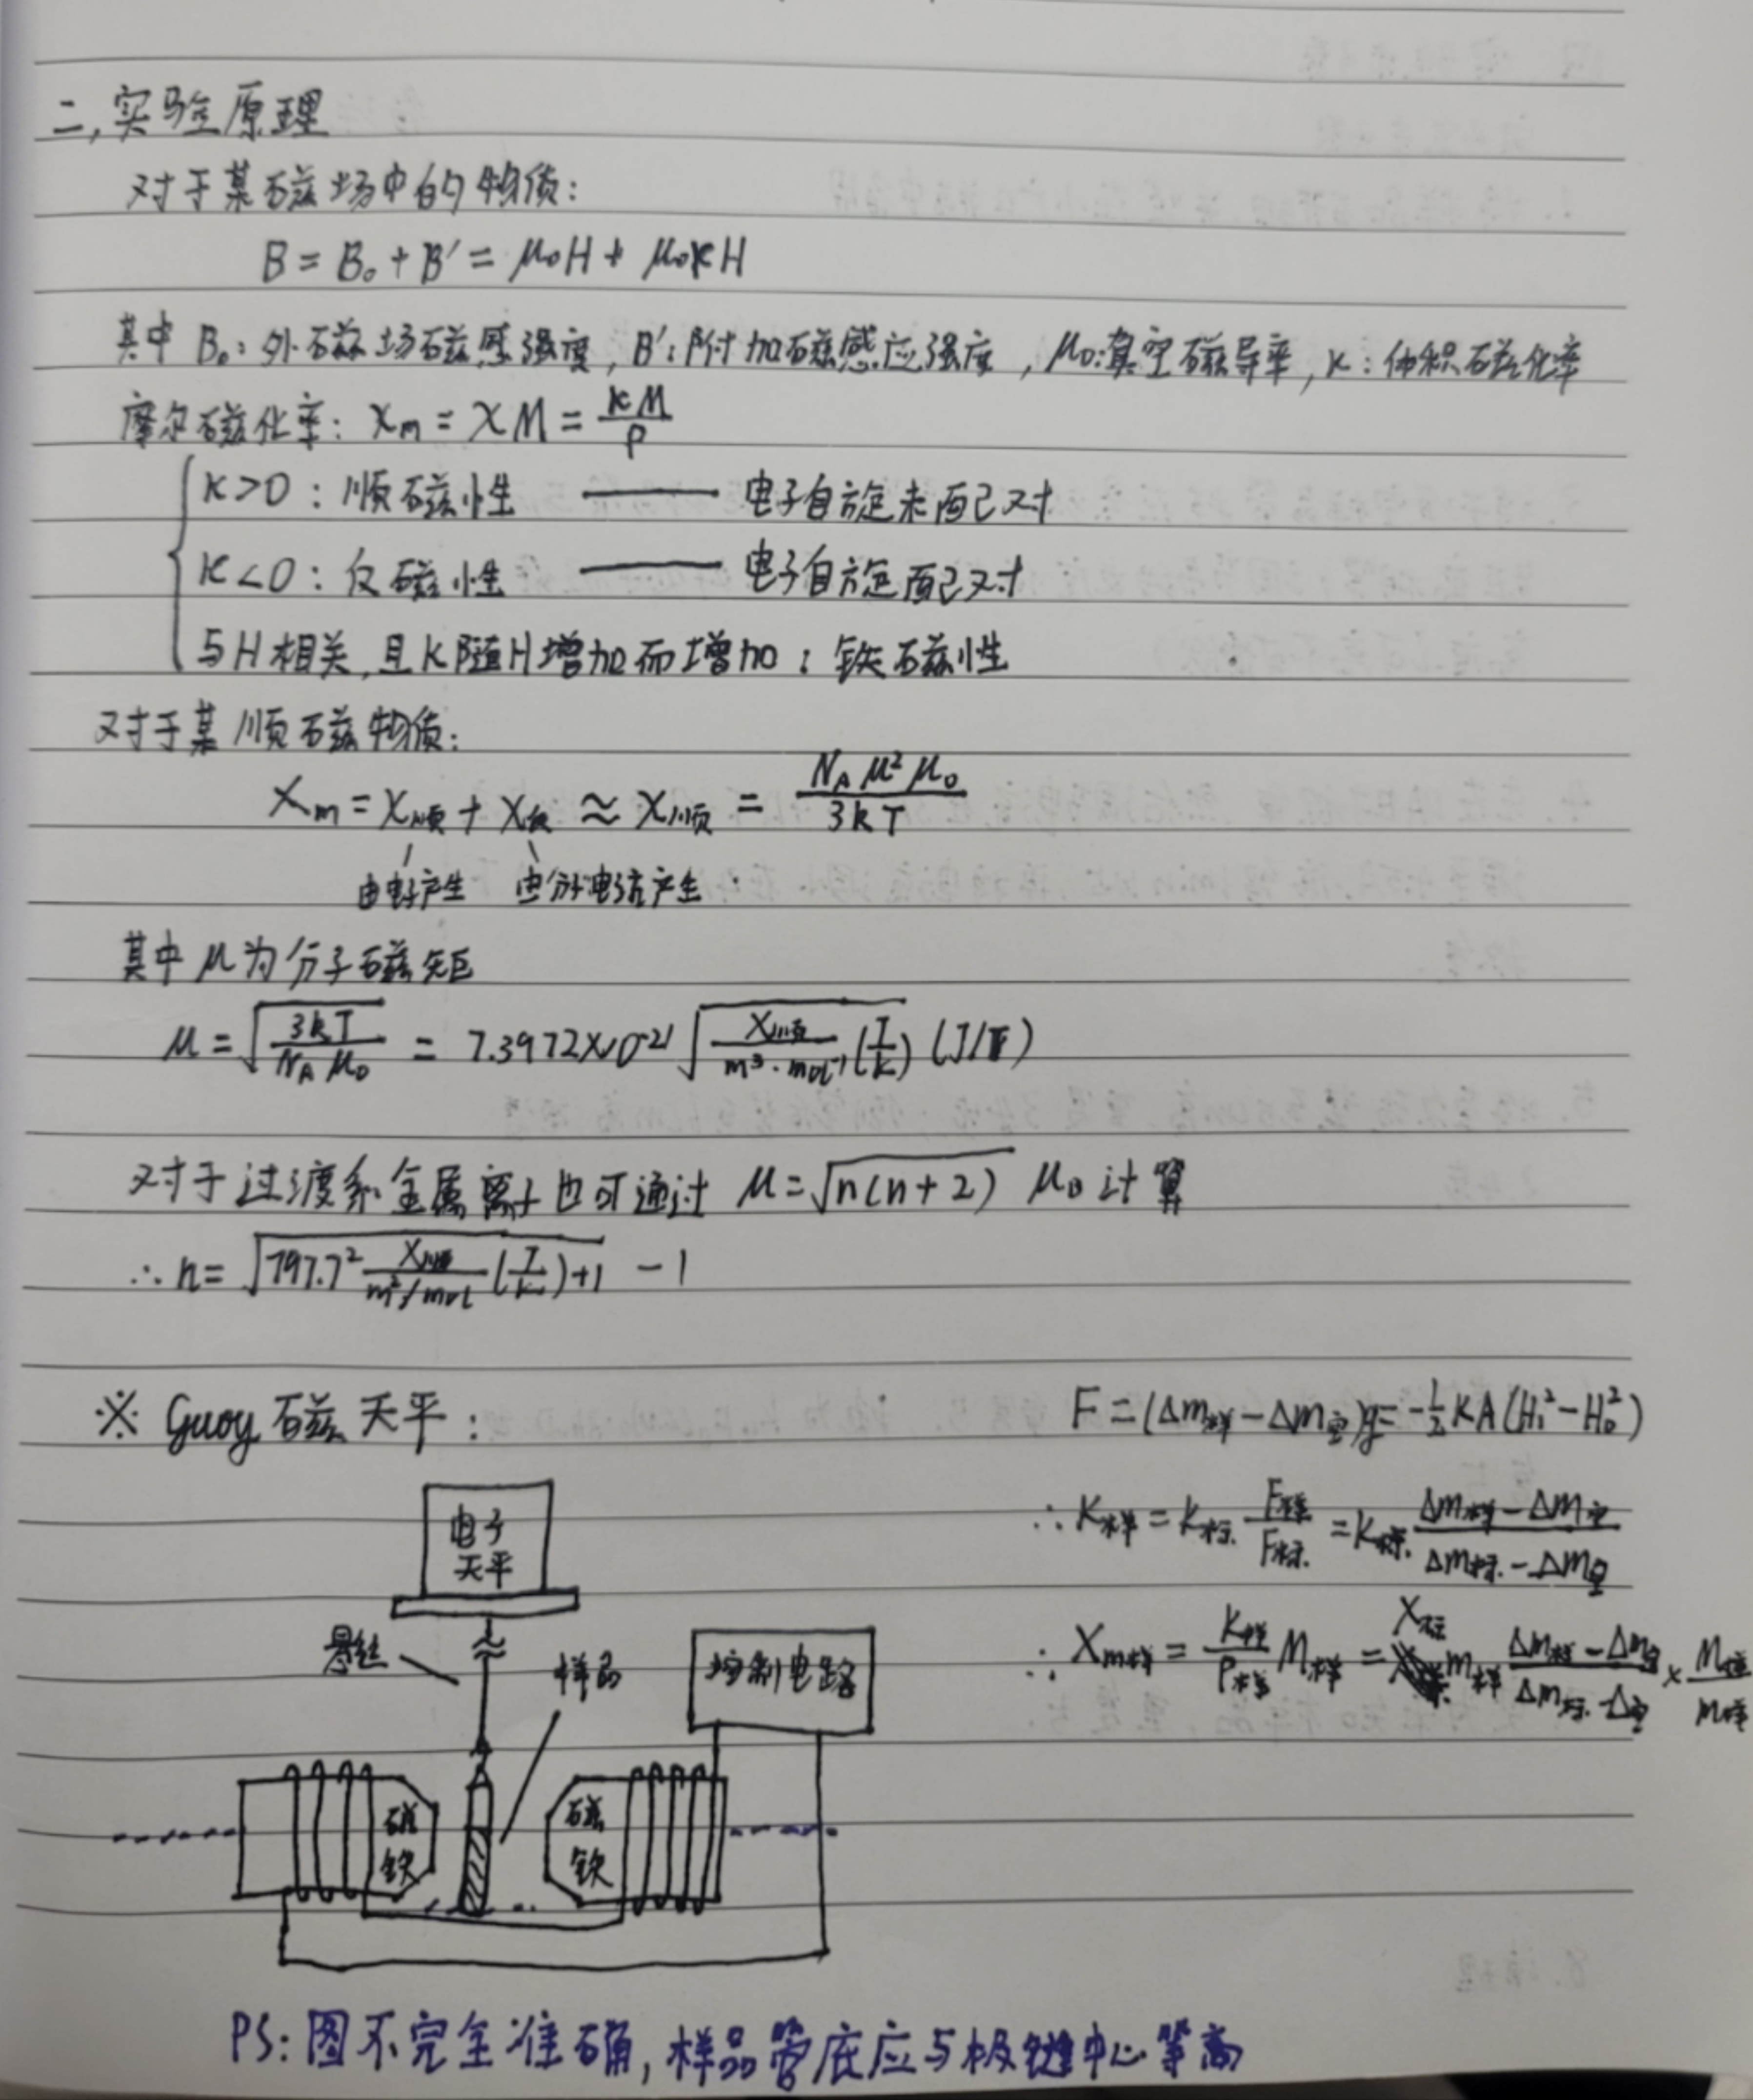
\includegraphics[width=0.6\textwidth]{1.png}
			\bicaption{实验预习报告的实验原理部分}{The principle part of the experiment in the experiment preview report}
		\end{figure}
				特别需要说明,\textbf{图1}中绘制的Guoy示意图有误,因为磁铁以高度中心为界磁场方向不同,为保证样品不受影响,样品管底不得低于极缝中心。


               
	\vbox{} % 设置空行
	     
    \section{实验部分}
    	\subsection{仪器和试剂}
    		仪器:\ \  磁天平(Guoy天平),研钵,试管;\par
			试剂:\ \  莫尔盐 (AR),$\rm{CuSO_{4}·5H_{2}O}$、$\rm{K_{4}Fe(CN)_{6}·3H_{2}O}$,未知样品;\par
    			
    	 \subsection{实验内容}
			\subsubsection{仪器预热与试剂准备}
				首先将天平的励磁电流调为0,电流细调旋钮左旋至最小并打开天平预热。将实验所需用到的摩尔盐、$\rm{CuSO_{4}·5H_{2}O}$、$\rm{K_{4}Fe(CN)_{6}·3H_{2}O}$以及样品用研钵研细,装在广口瓶中备用(实际操作中是直接装在研钵中备用,原因是本实验中所用的试剂均不易被氧化,若为易被氧化的试剂需储存在非敞口容器中。)
			\subsubsection{测量空管质量}
				将干净的空样品管挂在天平的悬钩上,调节磁铁位置使得样品管与两极距离相等,调整悬挂样品管的铜丝使得样品管的底部恰好位于极缝中心(此处可略高,但绝对不可低于极缝)。\par
				待天平数据不再变化,记录励磁电流为0\ A时的试管净重$m_{0}$,调节励磁电流至3\ A和4\ A,并记录相应的重量。将电流调节至4.5\ A并停留至少1min,随后再将电流调小记录试管在4\ A、3\ A和0\ A下的质量。
			\subsubsection{测量摩尔盐}
				将摩尔盐粉末装入样品管至5\ cm高,与测量空管相同,分别测量录励磁电流为0\ A、3\ A和4\ A时的试管总重$m$,将电流调节至4.5\ A并停留至少1min,随后再将电流调小记录试管在4\ A、3\ A和0\ A下的质量。测量完毕后,将试管倒空,按照同样的方法将样品装至6\ cm,重新测量。
			\subsubsection{测量$\rm{CuSO_{4}·5H_{2}O}$和$\rm{K_{4}Fe(CN)_{6}·3H_{2}O}$}
				与将样品分别换为$\rm{CuSO_{4}·5H_{2}O}$和$\rm{K_{4}Fe(CN)_{6}·3H_{2}O}$,重复2.2.3中的操作。
			\subsubsection{测量未知样品}
				取未知样品,实验者取的未知样品2号。重复2.2.3的操作两次。
			\subsubsection{计算与统计数据}
				计算每组数据的$\Delta m$,并记录。
    	
	
	 \section{数据与结果}
 		\subsection{实验数据记录及处理}
 			\subsubsection{试验记录}
				实验测量得到的数据如\textbf{表1}所示:
		 		
		 		% 插入表格示例
		 		  \begin{table}[!htbp]
					\arrayrulecolor{Maroon}
		 			\centering
		 			\zihao{5}
		 			\bicaption{实验数据}{Experimental data}
		 			\begin{tabular}{c c c c c c c c c c} 
		 				\toprule
		 				\multicolumn{3}{c}{励磁电流/A} 														& 0 	& 3 	& 4 	& 4.5  	& 4		& 3		& 0	\\
		 				%表格分行示例 不需要请删去
		 				\midrule
		 				\multirow{3}*{空管}						&						& B/mT 				& 4.1 	& 259.3	& 345.9 & /		&344.3	&260.9	&4.2	\\
		 														&						& m/g 				&8.5768 &8.5754	&8.5746 & /		&8.5748	&8.5756	&8.5770	\\
		 														&						&$\Delta\rm{m/g}$ 	& 	 	&-0.0014&-0.0022& /		&-0.0020&-0.0012&0.0002	\\
						\midrule
						\multirow{6}*{摩尔盐}					&\multirow{3}*{5\ cm}	& B/mT 				& 3.9 	& 253.2	& 335.9 & /		&337.0	&254.6	&3.7	\\
		 														&						& m/g 				&10.8498&10.8981&10.9338& /		&10.9343&10.8985&10.8944\\
		 														&						& $\Delta \rm{m/g}$ & 	 	&0.0483	&0.0840	& /		&0.0845	&0.0487	&0.0001	\\
						\cmidrule(lr){3-10}
																&\multirow{3}*{6\ cm}	& B/mT 				& 3.3 	& 254.3	& 336.4 & /		&336.9	&254.4	&3.5	\\
		 														&						& m/g 				&11.3233&11.3736&11.4102& /		&11.4103&11.3736&11.3237\\
		 														&						& $\Delta \rm{m/g}$ & 	 	&0.0503 &0.0869 & /		&0.0870 &0.0503 &0.0004	\\
						\midrule
						\multirow{6}*{$\rm{CuSO_{4}·5H_{2}O}$}	&\multirow{3}*{5\ cm}	& B/mT 				& 3.5 	& 253.0	& 335.6 & /		&336.8	&254.4	&3.4	\\
		 														&						& m/g 				&11.0390&11.0466&11.0522& /		&11.0525&11.0468&11.0391\\
		 														&						& $\Delta \rm{m/g}$	& 	 	&0.0076 &0.0132 & /		&0.0135	&0.0078	&0.0001	\\
						\cmidrule(lr){3-10}
																&\multirow{3}*{6\ cm}	& B/mT 				& 3.4 	& 252.8	& 335.4 & /		&336.2	&254.4	&3.4	\\
																&						& m/g 				&11.4748&11.4826&11.4886& /		&11.4888&11.4829&11.4749\\
																&						& $\Delta \rm{m/g}$	& 	 	&0.0078 & 0.0138& /		&0.0140	&0.0081	&0.0001	\\
						\midrule
						\multirow{6}*{$\rm{K_{4}Fe(CN)_{6}·3H_{2}O}$}	&\multirow{3}*{5\ cm}	& B/mT 		& 3.4 	& 252.6	& 335.3 & /		&336.7	&254.2	&3.6	\\
																&						& m/g 				&10.5895&10.5879&10.5866& /		&10.5863&10.5876&10.5894\\
																&						&$\Delta \rm{m/g}$	& 	 	&-0.0016&-0.0029& /		&-0.0032&-0.0019&-0.0001\\
						\cmidrule(lr){3-10}
																&\multirow{3}*{6\ cm}	& B/mT 				& 3.5 	& 252.5	& 335.6 & /		&335.3	&253.8	&3.5	\\
																&						& m/g 				&11.1490&11.1475&11.1460& /		&11.1461&11.1476&11.1493\\
																&						&$\Delta \rm{m/g}$	& 	 	&-0.0015&-0.0030& /		&-0.0029&-0.0014&0.0003	\\
						\midrule
						\multirow{12}*{未知样品}				&\multirow{3}*{5\ cm}	& B/mT 				& 3.4 	& 252.5	& 335.7 & /		&336.3	&254.2	&3.4	\\
																&						& m/g 				&10.7155&10.7245&10.7314& /		&10.7316&10.7247&10.7155\\
																&						&$\Delta \rm{m/g}$	& 	 	& 0.0090&0.0159	& /		&0.0161	&0.0092	&0.0000	\\
						\cmidrule(lr){3-10}
																&\multirow{3}*{6\ cm}	& B/mT 				& 3.4 	& 252.9	& 335.4 & /		&336.0	&254.0	&3.3	\\
																&						& m/g 				&11.1280&11.1375&11.1447& /		&11.1448&11.1377&11.1281\\
																&						&$\Delta \rm{m/g}$	& 	 	& 0.0095&0.0167	& /		&0.0168	&0.0097	&0.0001	\\
						\cmidrule(lr){3-10}
																&\multirow{3}*{5\ cm}	& B/mT 				& 3.3 	& 252.6& 335.6 & /		&336.3	&253.5	&3.4	\\
																&						& m/g 				&10.8190&10.8282&10.8351& /		&10.8351&10.8282&10.8190\\
																&						&$\Delta \rm{m/g}$	& 	 	&0.0092	&0.0161	& /		&0.0161	&0.0092	&0.0000	\\
						\cmidrule(lr){3-10}
																&\multirow{3}*{6\ cm}	& B/mT 				& 3.4 	& 252.9	& 335.6 & /		&336.9	&254.2	&3.3	\\
																&						& m/g 				&11.2247&11.2351&11.2429& /		&11.2432&11.2356&11.2246\\
																&						&$\Delta \rm{m/g}$	& 	 	&0.0104	&0.0182	& /		&0.0185	&0.0109	&0.0001	\\

						\bottomrule
						\end{tabular}
		 		\end{table}
		 		%\vbox{}
	 		\subsubsection{计算$\rm{CuSO_{4}·5H_{2}O}$和$\rm{K_{4}Fe(CN)_{6}·3H_{2}O}$的摩尔比磁化率}

			笔者实验时间为上午十点至下午三点,其中上午温度为\qty{25.6}{\degreeCelsius},下午温度为\qty{29.8}{\degreeCelsius}。
			考虑到主要的实验测量均在下午进行,这里采用\qty{29}{\degreeCelsius}作为实验室温度,即302.15\ K。由此可以根据\textbf{公式(1)}算出,实验条件下摩尔盐的比磁化率为:\par

			$$X_{0}=\frac{9500\times10^{-9}}{T+1}\times4\pi=3.938\times10^{-7}\ \rm{m}^{3}/kg \eqno(1)$$ \par
			
			根据实验原理可知,待测样的摩尔比磁化率可以由\textbf{公式(2)}给出。\par

			$$X_{m,a}=X_{0}M_{a}\frac{\Delta m_{a}-\Delta m_{e}}{\Delta m_{0}-\Delta m_{e}}\times\frac{m_{0}}{m_{a}} \eqno(2)$$\par
			将对应数值带入后计算得到的$X_{m,a}$在\textbf{表(2)}中给出:\par
			%表2
			\begin{table}[!htbp]
				\arrayrulecolor{Maroon}
				 \centering
				 \zihao{5}
				 \bicaption{$\rm{CuSO_{4}·5H_{2}O}$和$\rm{K_{4}Fe(CN)_{6}·3H_{2}O}$的摩尔比磁化率}{Molar susceptibility of copper sulfate pentahydrate and potassium ferricyanide}
				 \begin{tabular}{c c c c c c c c} 
					\toprule
					\multicolumn{2}{c}{磁化率} 									& $X_{3A}/10^{-8}\rm{m^{3}/mol}$	&$X_{4A}/10^{-8}\rm{m^{3}/mol}$	&$X_{4A}/10^{-8}\rm{m^{3}/mol}$	&$X_{3A}/10^{-8}\rm{m^{3}/mol}$\\
					\midrule
					\multirow{2}*{$\rm{CuSO_{4}·5H_{2}O}$}			&5\ cm    	& 1.644 	& 1.626		& 1.627 	&1.637\\
					 												&6\ cm		& 1.658		& 1.673		& 1.675 	&1.636\\
					\midrule
					\multirow{2}*{$\rm{K_{4}Fe(CN)_{6}·3H_{2}O}$}	&5\ cm    	& -0.152 	& -0.152	& -0.195	&-0.263\\
					 												&6\ cm		& -0.034 	& -0.139	& -0.199 	&-0.069\\
					\bottomrule
				\end{tabular}
			\end{table}
			
			对于计算数据取平均可知:
			$$X_{m,\rm{CuSO_{4}·5H_{2}O}}=1.637\times10^{-8}\rm{m^{3}/mol}$$
			$$X_{m,\rm{K_{4}Fe(CN)_{6}·3H_{2}O}}=-0.154\times10^{-8}\rm{m^{3}/mol}$$
			因为称量质量位于$\frac{1}{3}$量程附近,因此可认为允差$e_{m}$为0.7\ mg。根据\textbf{公式(3)}、\textbf{公式(4)}可以算出$X_{m,a}$的不确定度,即标准偏差。\par
			$$\sigma_{\Delta m}= \sqrt{2}\frac{e_{m}}{\sqrt{3}} = 0.6\ mg \eqno(3)$$
			$$\sigma_{X_{m,a}}= \frac{\Delta m_{a}-\Delta m_{e}}{\Delta m_{0}-\Delta m_{e}}\frac{m_{0}}{m_{a}}\times \sqrt{(\frac{\sigma _{m_{0}}}{m_{0}})^{2}+(\frac{\sigma _{m_{a}}}{m_{a}})^{2}+(\frac{\sigma _{\Delta m_{0}-\Delta m_{e}}}{\Delta m_{0}-\Delta m_{e}})^{2}+(\frac{\sigma _{\Delta m_{a}-\Delta m_{e}}}{\Delta m_{a}-\Delta m_{e}})^{2}} \eqno(4)$$

			代入数据可知对于$\rm{CuSO_{4}·5H_{2}O}$,$X_{m}$的标准偏差为0.019$\times10^{-8}\rm{m^{3}/mol}$,对于$\rm{K_{4}Fe(CN)_{6}·3H_{2}O}$,$X_{m}$的标准偏差为0.064$\times10^{-8}\rm{m^{3}/mol}$。因此可以得到:\par
			$$X_{m,\rm{CuSO_{4}·5H_{2}O}}=(1.637\pm0.019)\times10^{-8}\rm{m^{3}/mol}$$
			$$X_{m,\rm{K_{4}Fe(CN)_{6}·3H_{2}O}}=(-0.154\pm0.064)\times10^{-8}\rm{m^{3}/mol}$$

	 		\subsubsection{计算$\rm{CuSO_{4}·5H_{2}O}$和$\rm{K_{4}Fe(CN)_{6}·3H_{2}O}$的成单电子数} 
	 			根据\textbf{公式(5)}可以算出$\rm{CuSO_{4}·5H_{2}O}$和$\rm{K_{4}Fe(CN)_{6}·3H_{2}O}$的成单电子数。\par
				$$n=\sqrt{797.7^{2}\frac{X_{m,a}}{\rm{m^{3}/mol}}\frac{T}{K}+1}-1 \eqno(5)$$ \par
				因此可知:\par
				$$n_{\rm{CuSO_{4}·5H_{2}O}}=1.036$$
				$$n_{\rm{K_{4}Fe(CN)_{6}·3H_{2}O}}=-0.161$$ \par

				在$\rm{CuSO_{4}·5H_{2}O}$中,Cu(II) 的 d 电子排布为$(b_{1g})^{1}(a_{1g})^{2}(b_{2g})^2(e_{g})^{4}$,有 1 个单电子,与实验测得的结果是相吻合的。
				而测得黄血盐为抗磁性,此时不可用\textbf{公式(5)}来计算,得到的$n_{\rm{K_{4}Fe(CN)_{6}·3H_{2}O}}$也没有实际意义。但其$X$趋近于零,说明黄血盐是反磁性物质,因此可认为黄血盐中的单电子数目为0。

	 		\subsubsection{计算未知样品的比磁化率}
	 			根据\textbf{公式(6)}可以算出未知样品的比磁化率。\par
				$$X_{a}=X_{0}\frac{\Delta m_{a}-\Delta m_{e}}{\Delta m_{0}-\Delta m_{e}}\times\frac{m_{0}}{m_{a}} \eqno(6)$$\par
				将对应数值带入后计算得到的$X_{a}$在\textbf{表(3)}中给出:\par
				%表3
				\begin{table}[!htbp]
					\arrayrulecolor{Maroon}
					 \centering
					 \zihao{5}
					 \bicaption{未知样品的比磁化率}{Molar susceptibility of unknown sample}
					 \begin{tabular}{c c c c c c c c} 
						\toprule
						\multicolumn{2}{c}{磁化率} 					& $X_{3A}/10^{-8}\rm{m^{3}/kg}$	&$X_{4A}/10^{-8}\rm{m^{3}/kg}$	&$X_{4A}/10^{-8}\rm{m^{3}/kg}$	&$X_{3A}/10^{-8}\rm{m^{3}/kg}$\\
						\midrule
						\multirow{4}*{未知样品}			&5\ cm    	&8.758 		& 8.788		& 8.809		&8.723\\
						 								&6\ cm		&8.938		&8.993		&8.995	 	&8.973\\
						\midrule
														&5\ cm    	& 8.747 	& 8.743		& 8.613 	&8.742\\
						 								&6\ cm		& 9.322		& 9.352		& 9.408 	&9.597\\
						\bottomrule
					\end{tabular}
				\end{table}
				对于计算数据取平均可知:
				$$X_{unkunown}=8.828\times10^{-8}\rm{m^{3}/kg}$$
				因为称量质量位于$\frac{1}{3}$量程附近,因此允差$e_{m}$为0.7\ mg。根据\textbf{公式(3)}、\textbf{公式(4)}可以算出$X_{m,a}$的不确定度,即标准偏差。$X_{unkunown}$的标准偏差为0.026$\times10^{-8}\rm{m^{3}/kg}$。因此可以得到:\par
				$$X_{unkunown}=(8.828\pm0.026)\times10^{-8}\rm{m^{3}/kg}$$
				与摩尔盐的磁化率的比值为 1:4.46。
 	
 	\section{讨论与结论}
		\subsubsection{实验误差}
		查阅文献\cite{dean1992lange}得:
		$$X_{m,\rm{CuSO_{4}·5H_{2}O}} = 1.835 \times 10^{-8} m^{3}/mol$$
		$$X_{m,\rm{K_{4}Fe(CN)_{6}·3H_{2}O}} = -2.165 \times 10^{-9} m^{3}/mol$$
		$$E = \frac{X_{test}-X_{real}}{X_{real}} \eqno(7)$$
		根据相对误差公式\textbf{(5)}可计算出相对误差为:
		$$E_{\rm{CuSO_{4}·5H_{2}O}} = -10.8\%$$
		$$E_{\rm{K_{4}Fe(CN)_{6}·3H_{2}O}} = 7.1\%$$
		\subsection{实验误差分析}
		可以看出本次实验的测量误差较大,主要原因有以下几点:
		\begin{enumerate}
			\item 实验中的温度并非恒定,而是在上午和下午分别测量的,因此样品受到温度影响较大。标准样品摩尔盐的测量在上午,而其余部分的测量在下午,这会导致标样的数值参考价值较低。
			\item 实验要求在装样时样品紧密程度一致,但实际操作中难以做到,样品紧密程度不一,本实验对未知样品进行了一组平行测试,但可以注意到即使装柱高度相同其质量也相差0.1g左右,这已经足以产生较大误差。而不同样品间粉末粗细明显不同,装柱的紧实程度也无法控制,这必然导致实验数据的误差较大。
			\item 实验中的励磁电流需要依靠人为调整,无法做到精确控制,导致记录时磁场强度不同。可以明显注意到虽然都是逼近某一特定电流,上行时的磁场偏小,下行时的磁场偏大,这也会导致实验数据的误差较大。
		\end{enumerate} \par
		个人认为其中温度与装填紧密程度为在成误差的主要因素。
 	 
 		\subsection{实验结论}
		本次实验通过Guoy天平测量了$\rm{CuSO_{4}·5H_{2}O}$、$\rm{K_{4}Fe(CN){6}·3H{2}O}$的摩尔比磁化率分别为$(1.637\pm0.019)\times10^{-8}\rm{m^{3}/mol}$,$(-0.154\pm0.064)\times10^{-8}\rm{m^{3}/mol}$,约含有1个和0个单电子。未知样的比磁化率为$(8.828\pm0.026)\times10^{-8}\rm{m^{3}/kg}$。本次实验测量的摩尔比磁化率数据误差较大,主要原因是实验中的温度不恒定,样品紧密程度不一致,以及励磁电流无法精确控制.

\vbox{}  
%参考文献
\bibliographystyle{unsrt}
\bibliography{cite}
\end{document}